Based on your description, here's a possible TikZ LaTeX code that generates a visually appealing diagram representing the given equations:
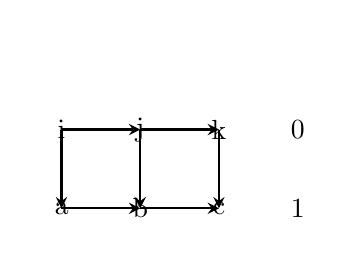
\begin{tikzpicture}
\begin{scope}[x=1cm,y=1cm]
% Draw the first equation
\node[white] at (0,0) {$i^2 + j^2 + k^2 = a^2$};
% Draw the second equation
\node[white] at (0,-1) {$i \cdot j \cdot k = ab$};
% Draw the third equation
\node[white] at (0,-2) {$i \cdot j \cdot k = ac$};
% Draw the letters and numbers
\node[black] at (-1,-1) {i};
\node[black] at (0,-1) {j};
\node[black] at (1,-1) {k};
\node[black] at (-1,-2) {a};
\node[black] at (0,-2) {b};
\node[black] at (1,-2) {c};
\node[black] at (2,-1) {0};
\node[black] at (2,-2) {1};
% Draw lines between the letters and numbers
\draw[-stealth,thick] (-1,-1) -- (-1,-2);
\draw[-stealth,thick] (0,-1) -- (0,-2);
\draw[-stealth,thick] (1,-1) -- (1,-2);
\draw[-stealth,thick] (-1,-1) -- (0,-1);
\draw[-stealth,thick] (0,-1) -- (1,-1);
\draw[-stealth,thick] (-1,-2) -- (0,-2);
\draw[-stealth,thick] (0,-2) -- (1,-2);
\end{scope}
\end{tikzpicture}
This code uses the `scope` environment to create a coordinate system for the diagram, and then draws the equations and letters/numbers using nodes and labels. The `\draw` command is used to draw lines between the letters and numbers to show their connections. The `-stealth` option adds arrowheads to the lines, and the `thick` option makes them thicker.
I hope this helps! Let me know if you have any other questions or if there